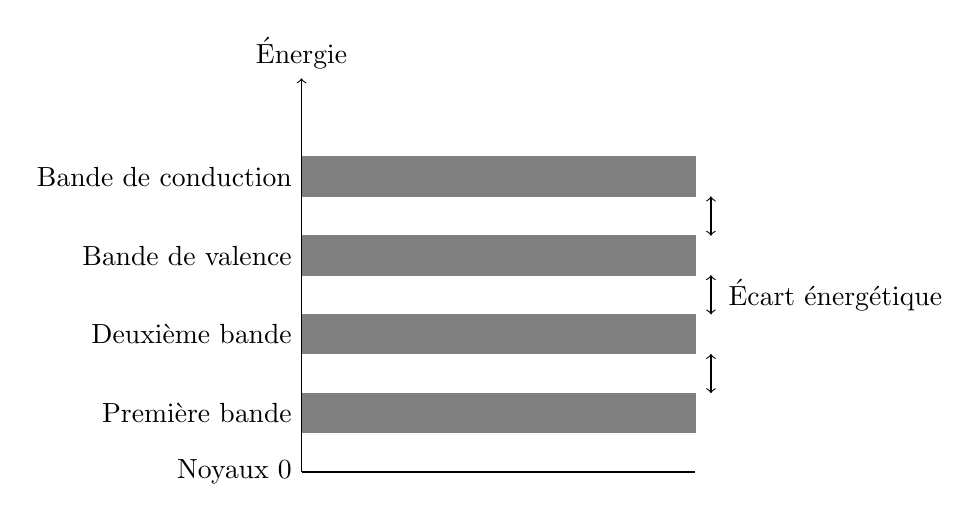
\begin{tikzpicture}
	
	\draw (0,0) -- (5,0);
	\draw[->] (0,0) -- (0,5);
	\filldraw[gray] (0.015,0.5) rectangle (5,1);
	\filldraw[gray] (0.015,1.5) rectangle (5,2);
	\filldraw[gray] (0.015,2.5) rectangle (5,3);
	\filldraw[gray] (0.015,3.5) rectangle (5,4);
	
	\draw (0,5) node[anchor=south] {Énergie};
	\draw (0,0) node[anchor=east] {Noyaux 0};
	\draw (0,0.75) node[anchor=east] {Première bande};
	\draw (0,1.75) node[anchor=east] {Deuxième bande};
	\draw (0,2.75) node[anchor=east] {Bande de valence};
	\draw (0,3.75) node[anchor=east] {Bande de conduction};
	
	\draw[<->] (5.2,1) -- (5.2,1.5);
	\draw[<->] (5.2,2) -- (5.2,2.5);
	\draw[<->] (5.2,3) -- (5.2,3.5);
	
	\draw (5.3,2.25) node[anchor=west] {Écart énergétique};
	
\end{tikzpicture}